\section{Diagrama Entidad-Relación}
\subsection{Diagrama Entidad-Relación}
\begin{figure}[H]
   \begin{center}
   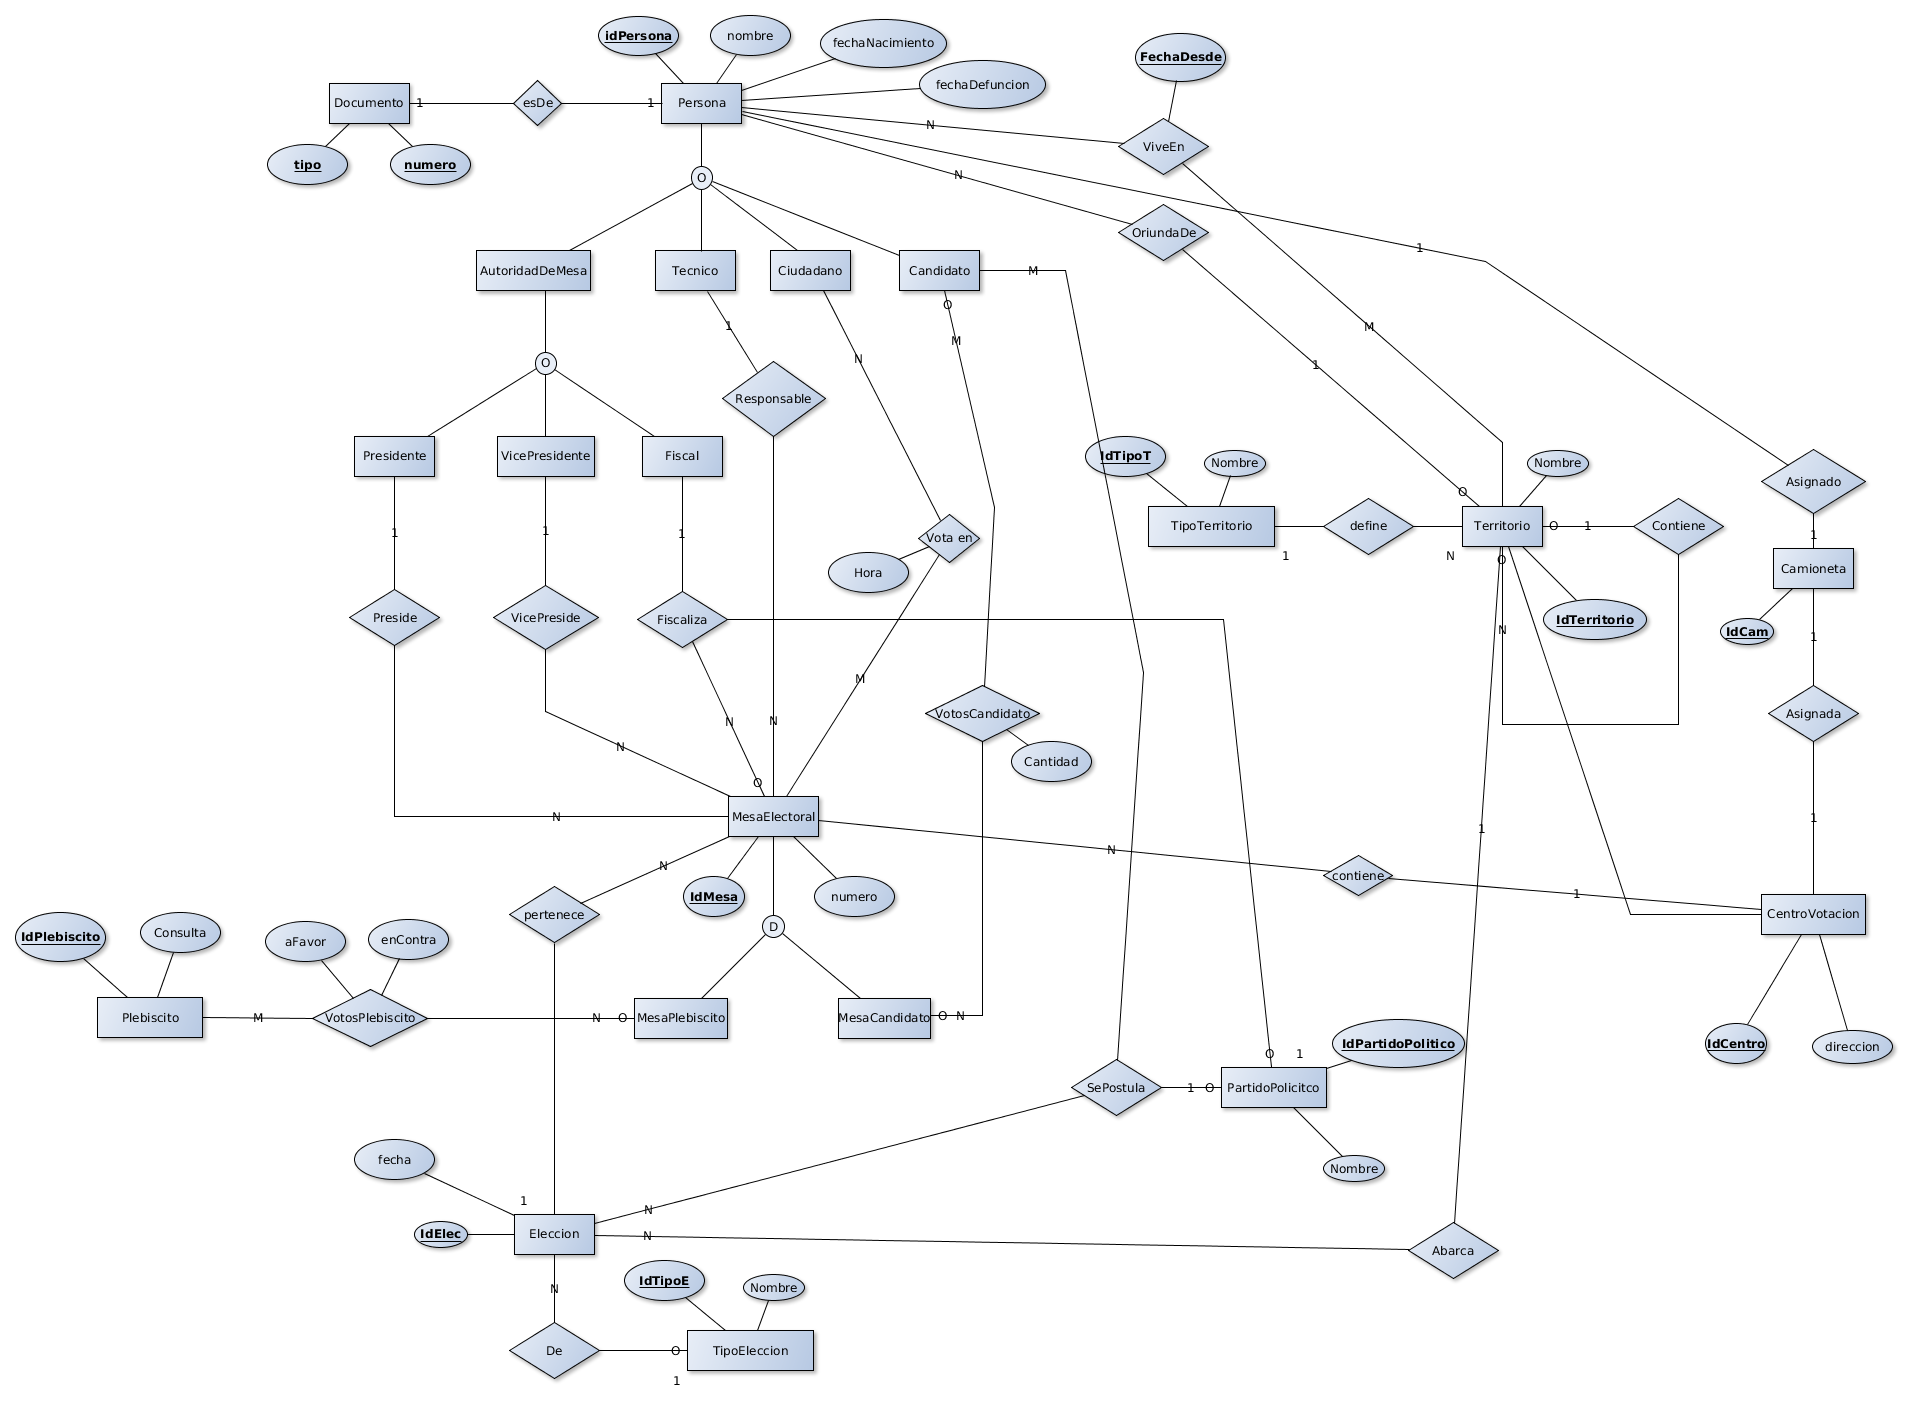
\includegraphics[angle=90,scale=0.32]{graphics/der.png}
   \caption{\textbf{Diagrama Entidad-Relación}}
   \label{fig:der}
   \end{center}
\end{figure}

\subsection{Restricciones Adicionales}

\subsubsection{Sobre los atributos}

\begin{itemize}
	\item{El número del Documento tiene que ser mayor a cero}.
	\item{El tipo del Documento tiene que ser alguno de los siguientes:
		\begin{itemize}
			\item{DNI}
			\item{CI}
			\item{LE}
			\item{LC}
		\end{itemize}
	}	
	\item{El atributo cantidad de la relación VotosCandidato tiene que ser mayor o igual a cero}

	\item{El atributo nombre de TipoTerritorio debe ser alguno de los siguientes y no se pueden repetir:
	  \begin{itemize}
	  	\item{País}
	  	\item{Provincia}
	  	\item{Localidad}
	  	\item{Ciudad}
	  \end{itemize}
	 }
	\item{El número de la MesaElectoral tiene que ser mayor a cero.}
	\item{Los  atributos aFavor y enContra de la relación VotosPlebiscito  tienen que ser mayor o igual a 0.}
	\item{El atributo fechaNacimiento no puede ser posterior al atributo fechaDefunción.}
\item{El atributo nombre de TipoEleccion debe ser alguno de los siguientes y no se pueden repetir:
	\begin{itemize}
		\item{Presidencial}
		\item{Gobernador}
		\item{Intendente}
		\item{Plebiscito}
	\end{itemize}
}

\item{Territorios sólo pueden contener a territorios más chicos:
\begin{itemize}
	\item{Un País sólo puede contener Provincias.}
	\item{Una Provincia sólo puede contener Localidades o Ciudades.}
	\item{Una Localidad sólo puede contener Ciudades.}
	\item{Una Ciudad no puede contener nada.}
\end{itemize}
}
\item{Sólo se puede ser oriundo de una ciudad.}
\item{El atributo fechaDesde de la relación ViveEn tiene que estar entre fechaNacimiento y fechaDefunción de la persona correspondiente.}

\item{Sólo los Territorios con TipoTerritorio de nombre "Ciudad" pueden participar de la relación OriundoDe.}
\item{Votar en las elecciones que corresponden según territorio.}

\item{Para que un Ciudadano pueda participar en VotosCandidato o VotosPlebiscito con la MesaElectoral correspondiente, ésta debe pertenecer a una Eleccion que abarque un Territorio el cual debe ser igual o contiene en algún nivel al Territorio en el cual el Ciudadano ViveEn en el momento de la elección.\footnote{Quien participa de ViveEn es Persona, no Ciudadano. Nos estamos refiriendo a la Persona correspondiente a dicho Ciudadano.}
}

%Presentarse como candidato para la elección de algún cargo.

\item{Para que un Candidato pueda participar de SePostula con un PartidoPolítico en una Eleccion, el Territorio que esta última abarca debe ser igual o contener en algún nivel al Territorio en el cual el Candidato debe participar en ViveEn\footnote{Idem [1] pero para Candidato.} con una fechaDesde mayor a los X años.
}

%Solamente reciben votos los candidatos que se presentan a la elección.

\item{Para que un Candidatos puede participar de VotosCandidato con MesaCandidato, debe participar en SePostula con la Elección a la cual la MesaElectoral pertenece.
}

%Si el Partido Político tiene fiscales, tiene que postularse.

\item{Para que PartidoPolítico participe de fiscaliza con una MesaElectoral, debe participar en sePostula con un Candidato en una Elección que contenga esa MesaElectoral.}

\item{Dentro de una Elección, los números de MesaElectoral no se pueden repetir.}

\item{Para cada elección, una Persona sólo puede ser Presidente, VicePresidente, Fiscal, Candidato o Técnico de manera disjunta.}

\item{Los Ciudadanos solo pueden ser Autoridad de la Mesa en que votan}

\item{Ciudadanos sólo pueden votarEn una única MesaElectoral por Elección.}

\item{No puede pasar que para una elección haya por lo menos una  MesasElectorales y por lo menos una MesaPlebiscito.}

\item{No hay más votos que votantes}

\item{Para cada MesaCandidato, la sumatoria de cantidad en cada tupla de VotoCandidato debe ser menor igual a la cantidad de tuplas en la relación VotaEn entre MesaElectoral y Ciudadano.}

\item{Para cada MesaPlebiscito, la sumatoria de aFavor y enContra en cada tupla de VotoPlebiscito debe ser menor igual a la cantidad de tuplas en la relación VotaEn entre MesaElectoral y Ciudadano.}

\item{Mayor de 16 para votar.}

\item{Para que una Persona sea Autoridad de Mesa tiene que tener más de 16 años.}

\item{Los muertos no votan}

\item{Para que un Ciudadano participe en VotaEn con una MesaElectoral, no debe tener fecha de defunción anterior a la fecha de la Elección correspondiente a esa Mesa.}

\item{No puede haber 2 o más  elecciones con misma fecha y mismo TipoEleccion para mismo Terrritorio.}

\item{El CentroVotacion tiene q estar en un territorio contenido en el de la eleccion y que ademas sea una ciudad.}


\end{itemize}


\subsection{Consideraciones}

\subsubsection{Acerca de las afiliaciones a los partidos políticos}

\begin{itemize}
\item{Hemos decidido no modelar las afiliaciones de las personas a los partidos políticos, no sólo porque podrían ser muchas tuplas, sino que no nos parece un aspecto central del problema a modelar.}

\item{Consideramos que las afiliaciones a los partidos políticos de fiscales y candidatos se entienden por sus participaciones en fiscaliza y sePostula, respectivamente.}
\end{itemize}

\subsubsection{Sobre el impedimento para postularse según lugar de nacimiento.}

\begin{itemize}
\item{Sabemos que ciertos cargos requieren que un candidato haya nacido en el territorio correspondiente a la elección, como por ejemplo la elección de Presidente.Sin embargo, esto no es requerido para todos los cargos políticos y por ese motivo no forzamos esa restricción.}
\end{itemize}
